\section {Performance Evaluation}

\begin{table}[t]
    \caption{Experiment Parameters}
    \centering
    \resizebox{7.5cm}{!}{
    \begin{tabular}{|c|c|}
    \hline
      Parameter & Value \\
    \hline
      Number of users $N$ & \{2, 3\} \\
      Number of antennas per user $L_{xu}$ & 1 \\
      Number of antennas at AP $L_y$ & \{2, 3, 4\} \\
      User to AP distance range $[d_{min}, d_{max}]$ & [1m, 10m]\\
      Channel bandwidth $W$ & 100 MHz \\
      Number of channel delay taps $n_{delay}$ & \{9, 18\} \\
      FFT length ${fft}_{length}$ & \{16, 32, 64, 128, 256\} \\
      SNR & [-10, 50] dB \\
    \hline
    \end{tabular}}
    \label{tab:experiment-parameters}
\end{table} 
\begin{figure}
    \centering
    \begin{subfigure}[b]{8cm}
    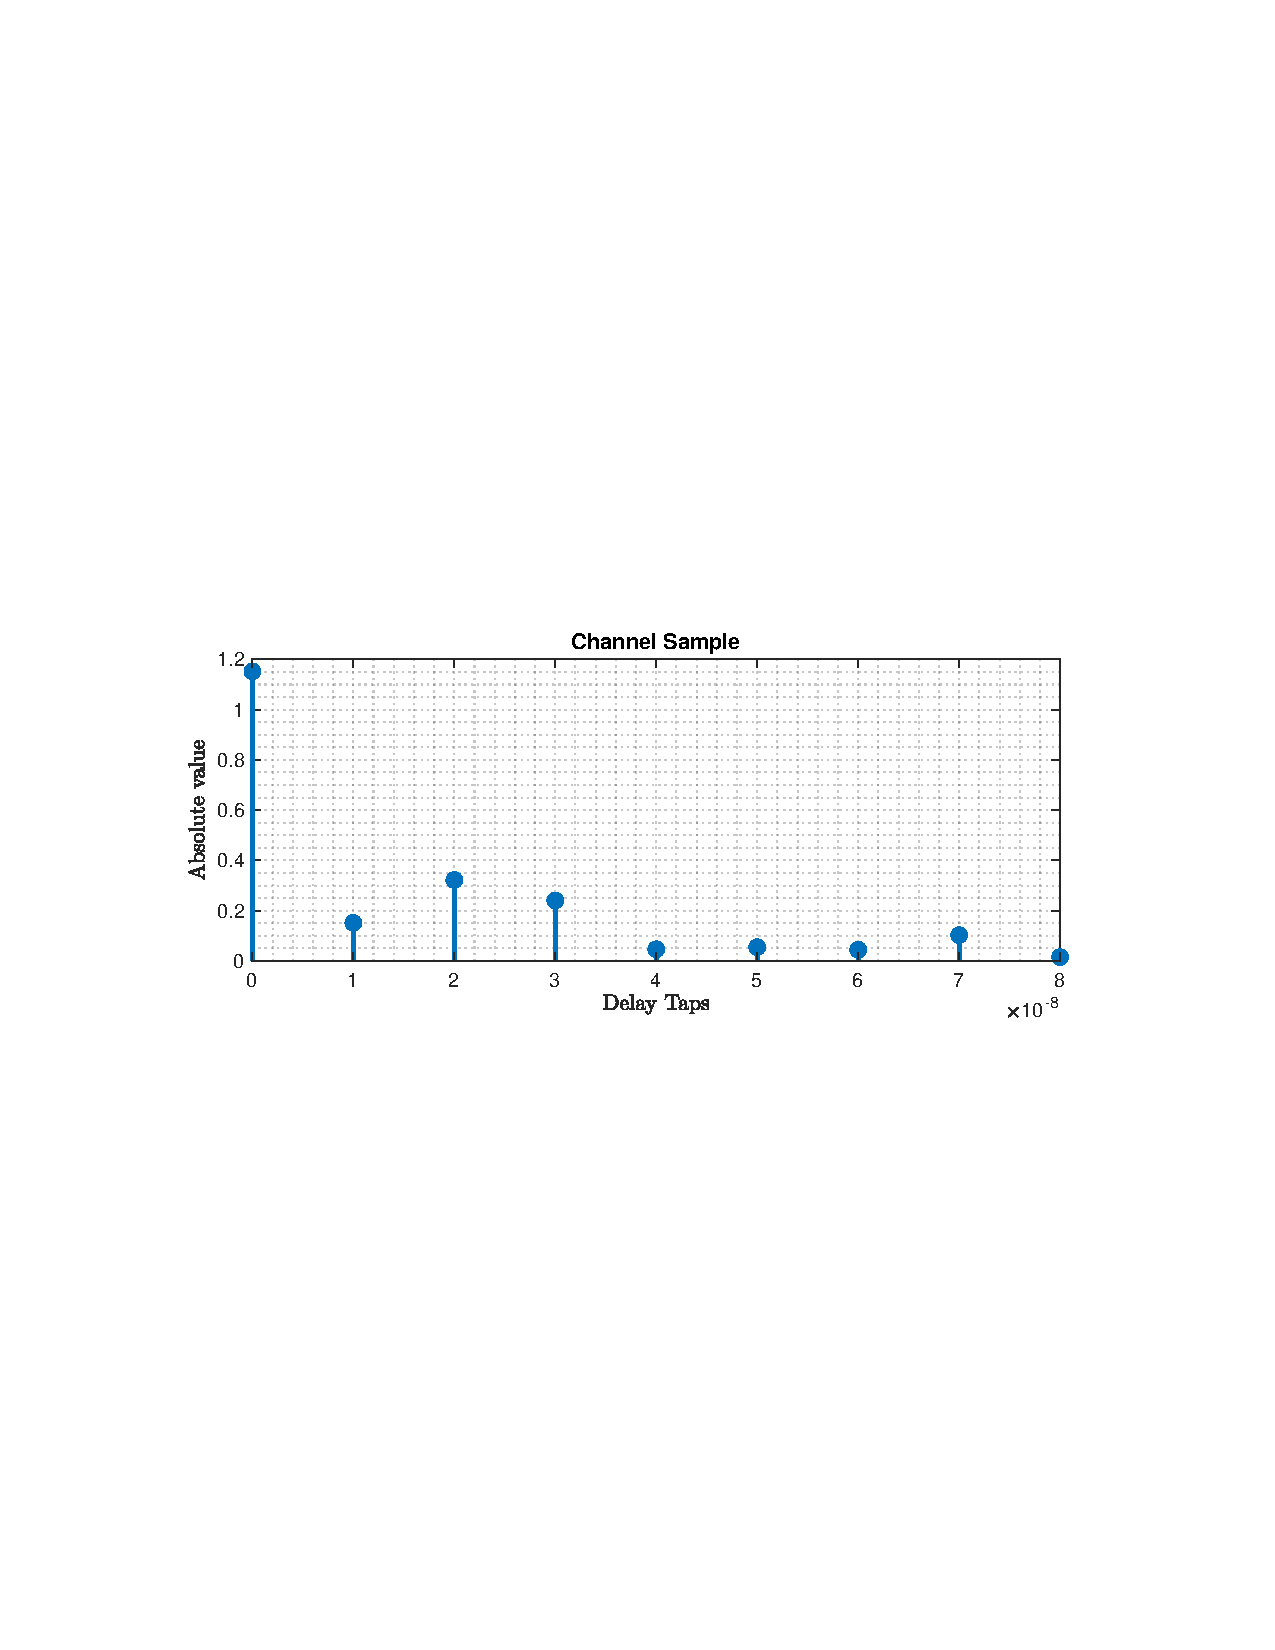
\includegraphics[trim={3cm 10.7cm 3cm 10cm},clip, width=8cm]{figures/TimeSample_2.pdf}
    \end{subfigure}
    \begin{subfigure}[b]{8 cm}
    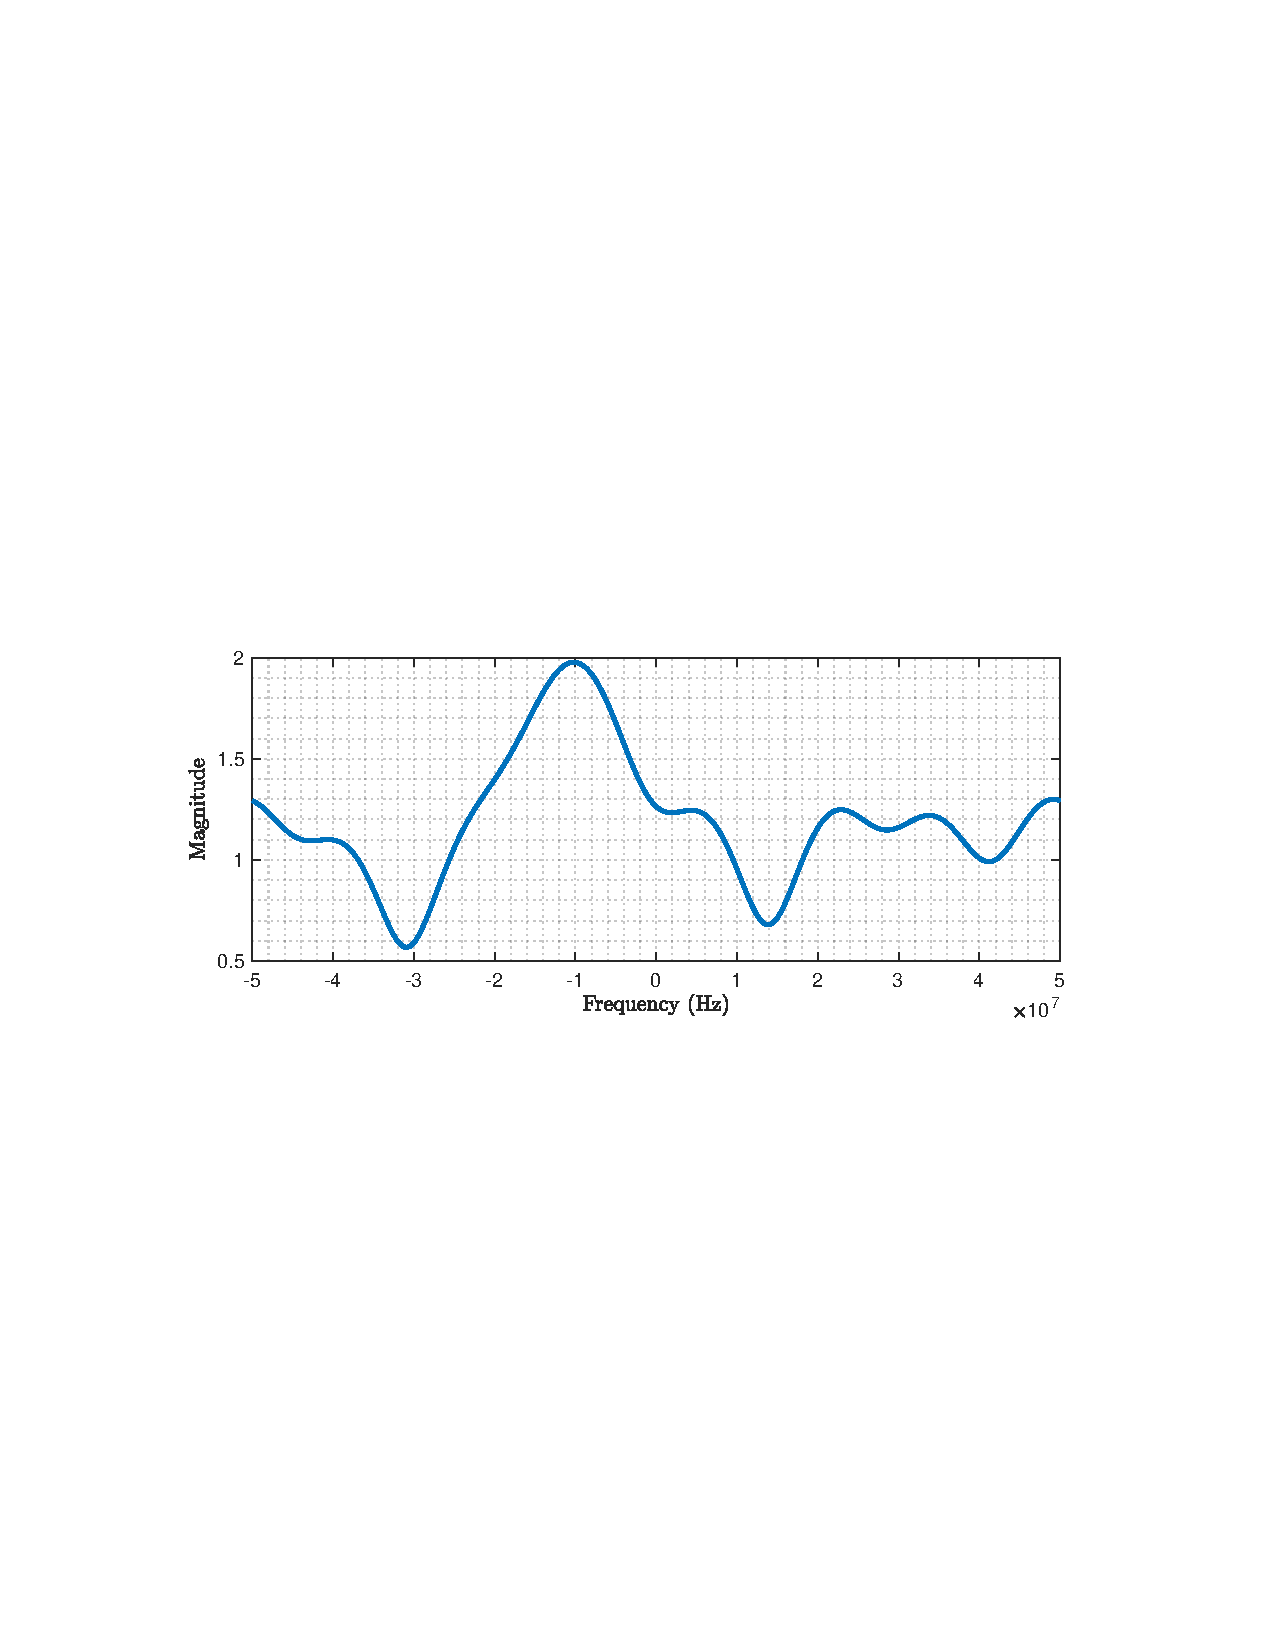
\includegraphics[trim={3cm 10.7cm 3cm 10cm},clip, width=8cm]{figures/FreqSample_2.pdf}   
    \end{subfigure}
    \caption{Channel B Samples}
    \label{fig:channel-samples}
\end{figure}

\begin{table}[t]
    \caption{Parameters for 2 Experiment Scenarios}
    \centering
    \resizebox{8.5cm}{!}{
    \begin{tabular}{|c|c|c|}
    \hline 
    \textbf{Parameter}& \textbf{Case 1}& \textbf{Case 2}\\
    \hline 
    \textbf{Antennas/user}& 1 & 1 \\
    \textbf{AP Antennas}& 2 & 2\\
    \textbf{Users}& 2 & 3 \\
    \textbf{Distance from AP (m)}& \{3, 3\} & \{3, 3, 3\} \\
    \hline
    \textbf{Data Rates (OFDM) (Mbps)}& \{239, 481\} & \{136, 236, 266\} \\
    \textbf{Data Rates (Proposed) (Mbps)}& \{239, 481\} & \{470, 470, 470\}\\
    \hline
    \textbf{Energy (OFDM)}& \{1, 1\} & \{1, 1, 1\} \\
    \textbf{Energy (Proposed)}& \{0.1168, 0.2870\} & \{0.3437, 0.9621, 0.9308\} \\
    \hline 
    \end{tabular}}
    \label{tab:scearios-single}
\end{table}


% \begin{table}[t]
% \caption{Energy Consumption versus Number of AP Antennas for Single Antenna Per User, $U = 3$, $L_{xu} = 1$, $\textrm{distance from AP} = \{3m,3m,3m\}$}
% \centering
% \begin{tabular}{|c|c|c|}
% \hline
% \multirow{2}{*}{\textbf{AP Antennas}} & \multicolumn{2}{c|}{\textbf{Average Energy}} \\ \cline{2-3} 
%                      & \textbf{ OFDM} & \textbf{GDFE}  \\ \hline
% 1                    & 1                             & 0.5383         \\ \hline
% 2                    & 1                             & 0.1246         \\ \hline
% 3                    & 1                             & 0.0898         \\ \hline
% 4                    & 1                             & 0.1401         \\ \hline
% \end{tabular}
% \label{tab:my_label}
% \end{table}



\begin{table}[t]
\caption{Energy Consumption versus Number of AP Antennas for Single Antenna Per User, $R = 201.702 \textrm{ Mbps}$, $U = 3$, $L_{xu} = 1$, $\textrm{distance from AP} = \{3m,3m,3m\}$}
\centering
\resizebox{9cm}{!}{
\begin{tabular}{|c|c|c|c|c|}
\hline
\multirow{2}{*}{\begin{tabular}[c]{@{}c@{}}\textbf{AP} \\ \textbf{Antennas}\end{tabular}} & \multicolumn{2}{c|}{\textbf{OFDM}} & \multicolumn{2}{c|}{\textbf{Proposed Algorithm}} \\ \cline{2-5} 
                     & \textbf{Energy}& \textbf{$\textrm{Energy}_{\textrm{avg}}$}& \textbf{Energy}& \textbf{$\textrm{Energy}_{\textrm{avg}}$}\\ \hline
1                    & [1,  1,  1] & 1& [0.5721,    0.5417,    1.1325]& 0.7488\\ \hline
2                    & [0.9, 0.9,  0.9] & 0.9& [0.1354,    0.0422,    0.1552]& 0.1109\\ \hline
3                    & [0.75, 0.75, 0.75] & 0.75& [0.0294,    0.0750,    0.0893]& 0.0646\\ \hline
4                    & [0.3, 0.3, 0.3] & 0.3& [0.0214,    0.0508,    0.0556]& 0.0426\\ \hline
\end{tabular}}
\label{tab:energy-compare}
\end{table}
\begin{table}[t]
\caption{Energy Consumption versus Number of AP Antennas for Single Antenna Per User, Fixed energy for OFDM, $U = 3$, $L_{xu} = 1$, $\textrm{distance from AP} = \{3m,3m,3m\}$}
\centering
\resizebox{9cm}{!}{
\begin{tabular}{|c|c|c|c|c|}
\hline
\multirow{2}{*}{\begin{tabular}[c]{@{}c@{}}\textbf{AP} \\ \textbf{Antennas}\end{tabular}} & \multicolumn{2}{c|}{\textbf{OFDM}} & \multicolumn{2}{c|}{\textbf{Proposed Algorithm}} \\ \cline{2-5} 
                     & \textbf{Energy}& \textbf{Data Rates}& \textbf{Energy}& \textbf{Data Rates}\\ \hline
1                    & [1,  1,  1] & [204,  174,  175]& [1.1534,    0.5194,    0.7641]& [204,  174,  175]\\ \hline
2                    & [1,  1,  1] & [224,   87,  210]& [0.0259,    0.1662,    0.1737]& [87,  164,  270]\\ \hline
3                    & [1,  1,  1] & [233,  117,  200]& [0.0233,    0.1171,    0.1223]& [18,   210,  322]\\ \hline
4                    & [1,  1,  1] & [290,  180,  252]& [0.1818,    0.1738,    0.0938]& [408,  202,  112]\\ \hline
\end{tabular}}
\label{tab:energy-compare2}
\end{table}
\begin{figure}[t]
    \centering
    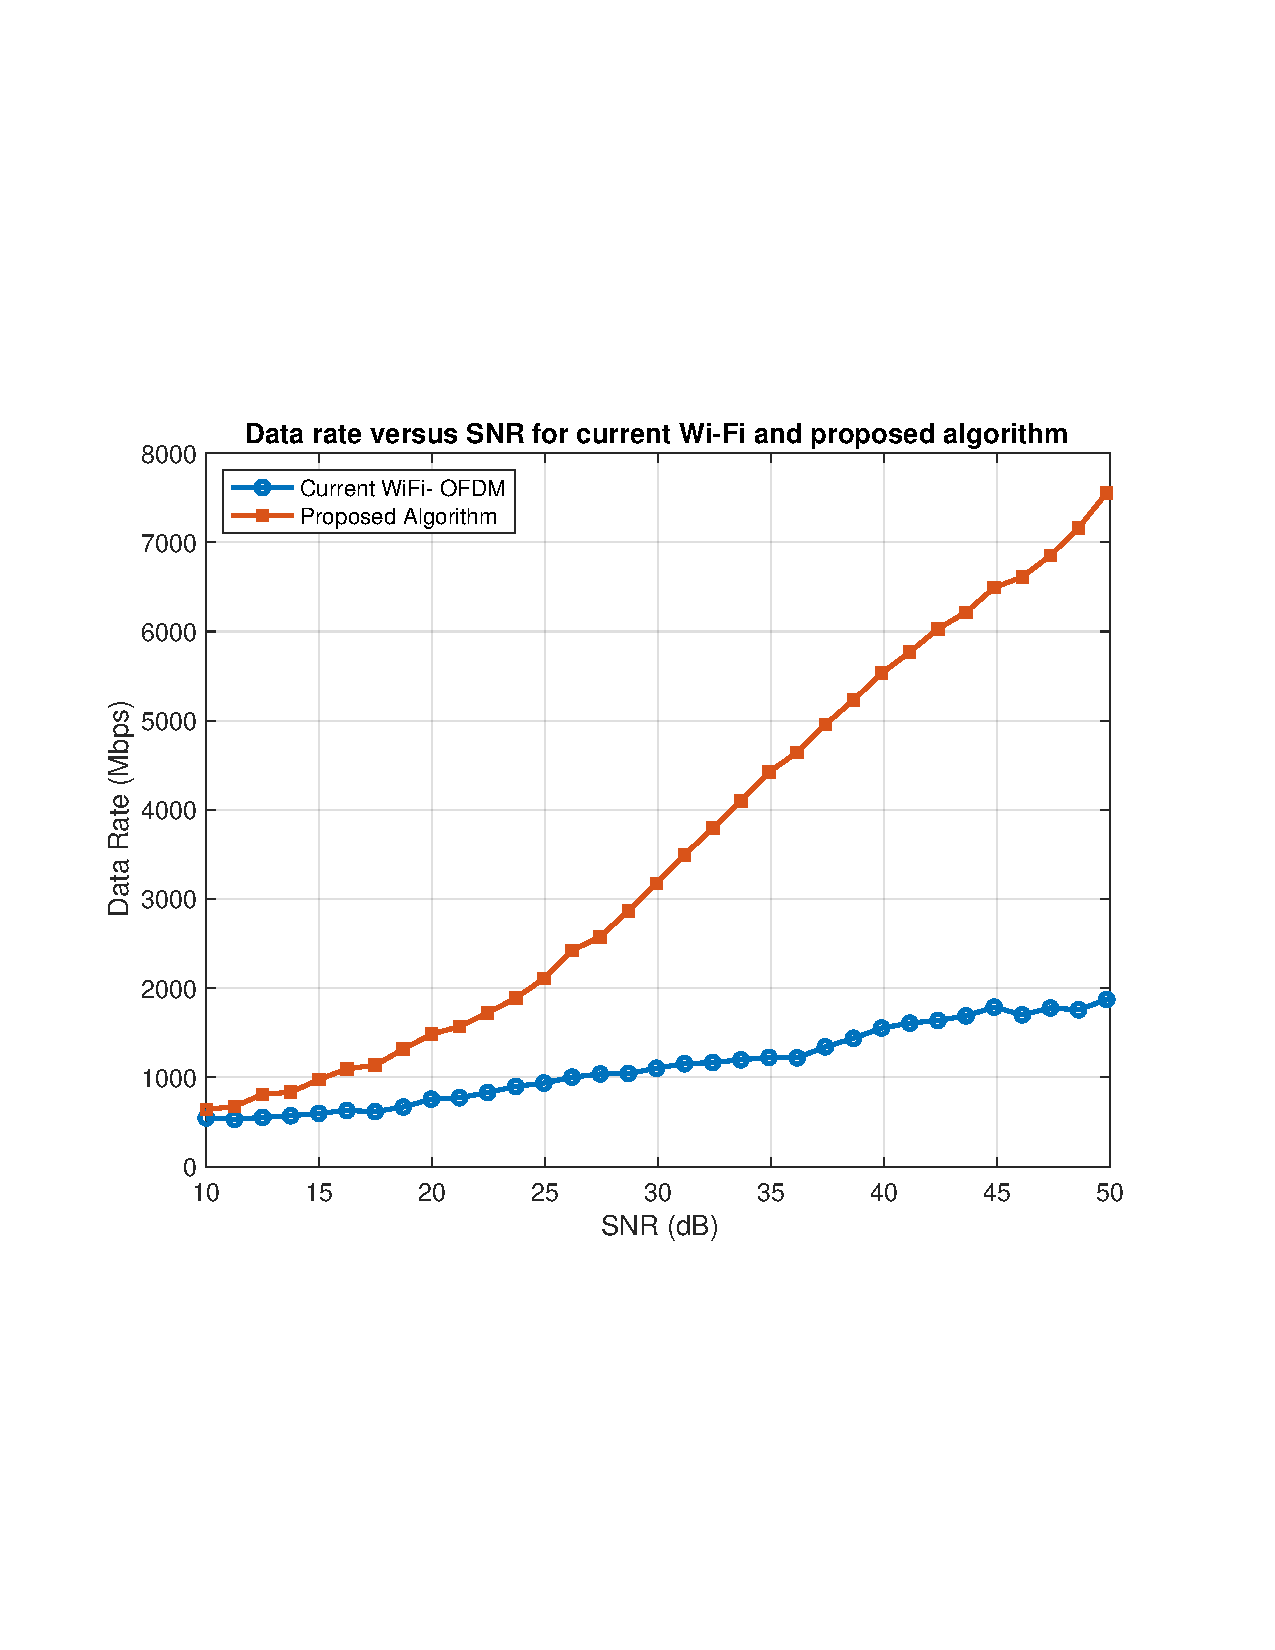
\includegraphics[trim = {30, 180, 10, 200}, clip, height = 6.3cm]{figures/data_rate_versus_SNR.pdf}
    \caption{Sum Rate versus SNR for Single Antenna Per User: Current Wi-Fi OFDM and Proposed Algorithm}
    \label{fig:data-rate-snr-single}
\end{figure}
\begin{figure}
    \centering
    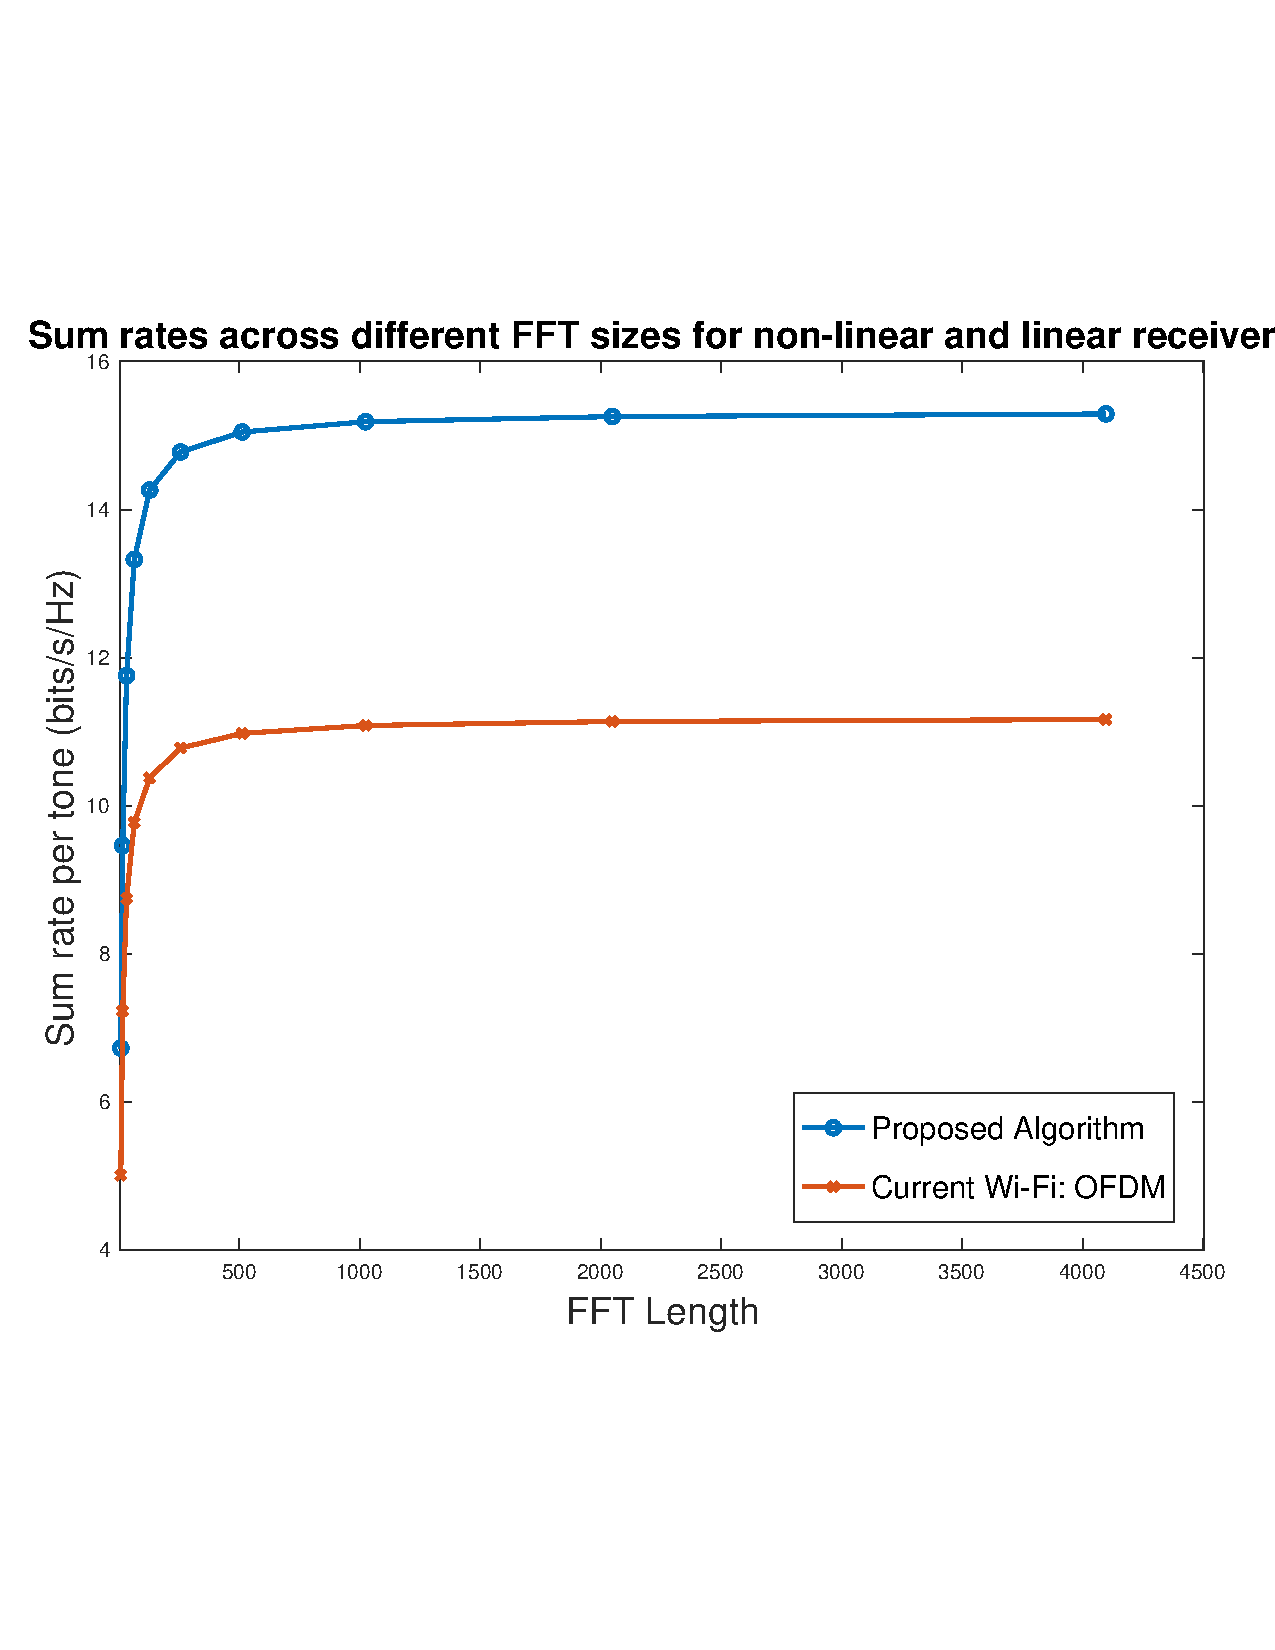
\includegraphics[trim = {0, 150, 0, 130}, clip, height = 7cm]{figures/3UsersEqualDistance3mSumRatePerTone.pdf}
    \caption{Sum rate versus FFT length for equidistant users with single antenna per user}
    \label{fig:data-rate-fft-single}
\end{figure}
\begin{figure}
    \centering
    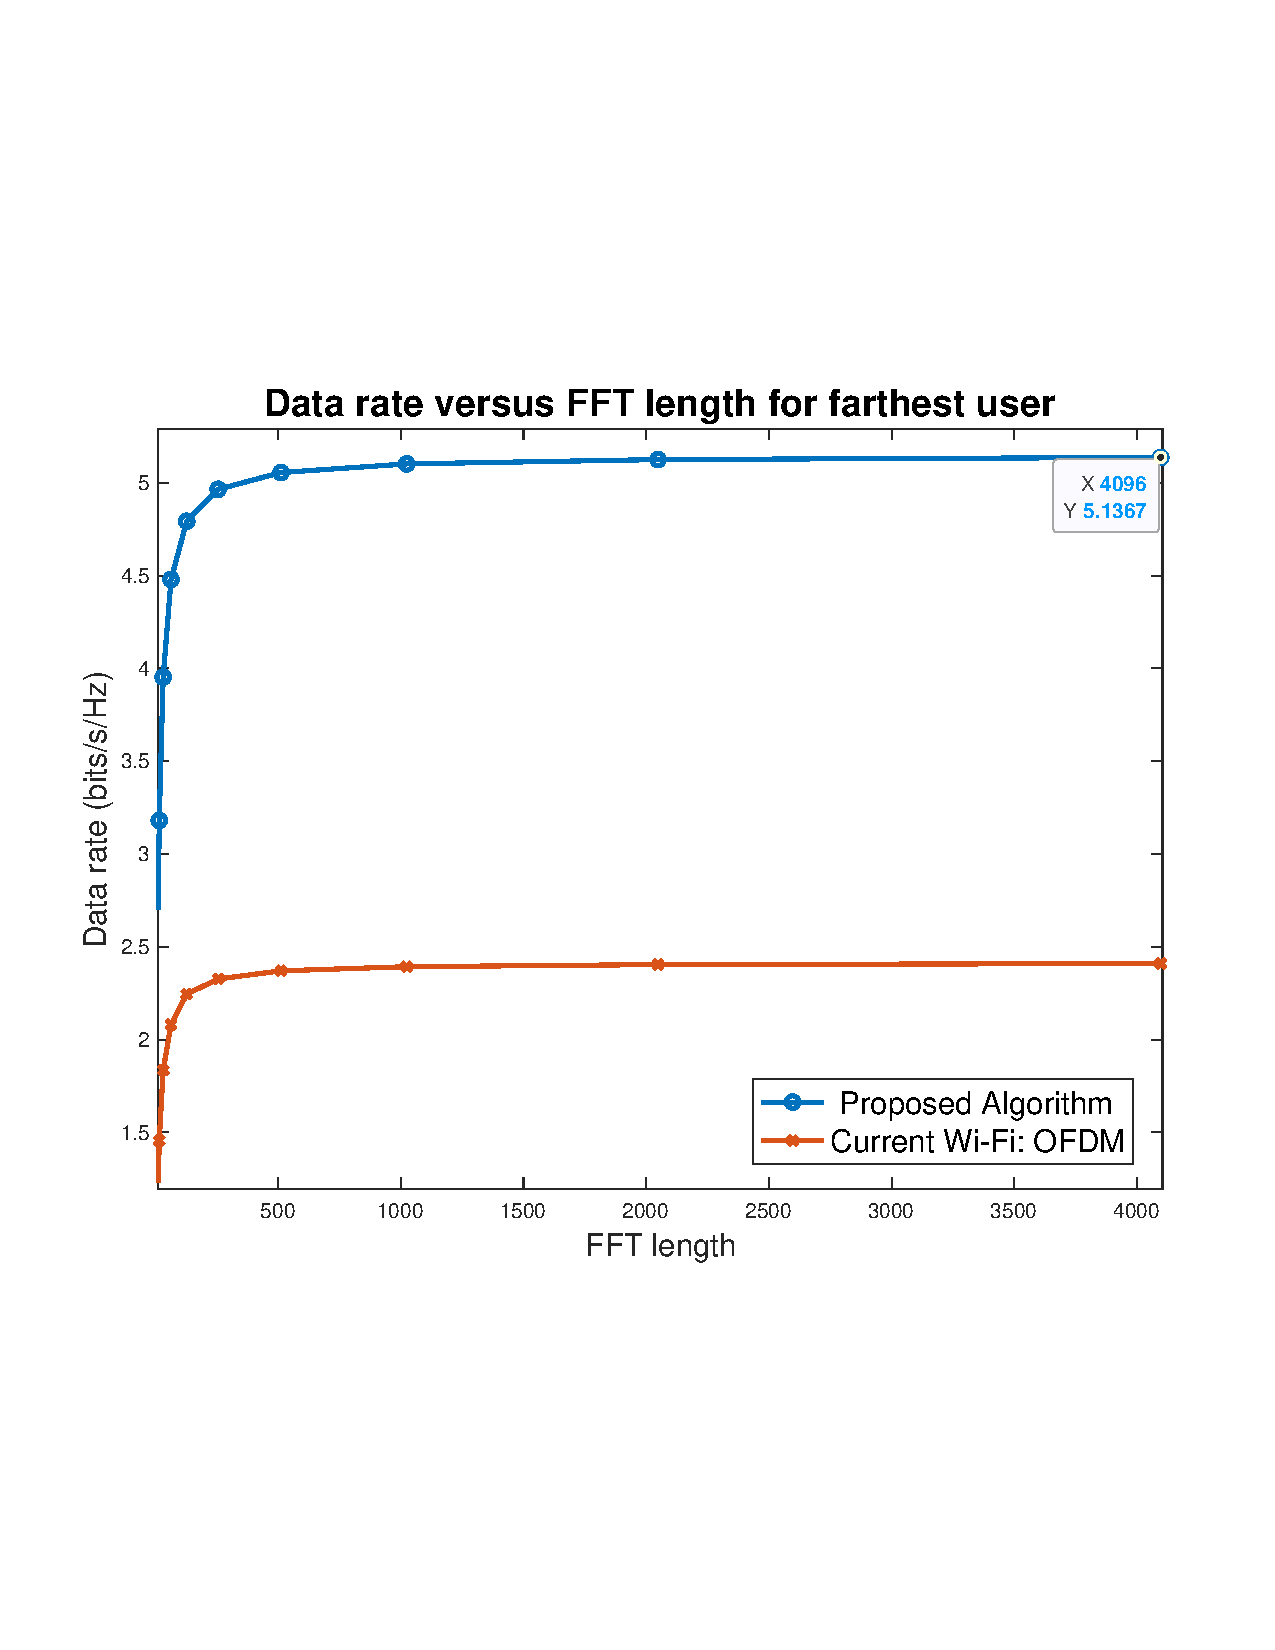
\includegraphics[trim = {20, 180, 0, 180}, clip, height = 7cm]{figures/3Users3_5_8mFarthestUserRatePerTone.pdf}
    \caption{Data rate versus FFT length for the farthest user with user distances from AP = \{3m, 5m, 8m\}, and single antenna per user}
    \label{fig:data-rate-farthest-fft-single}
\end{figure}
% \begin{figure}
%     \centering
%     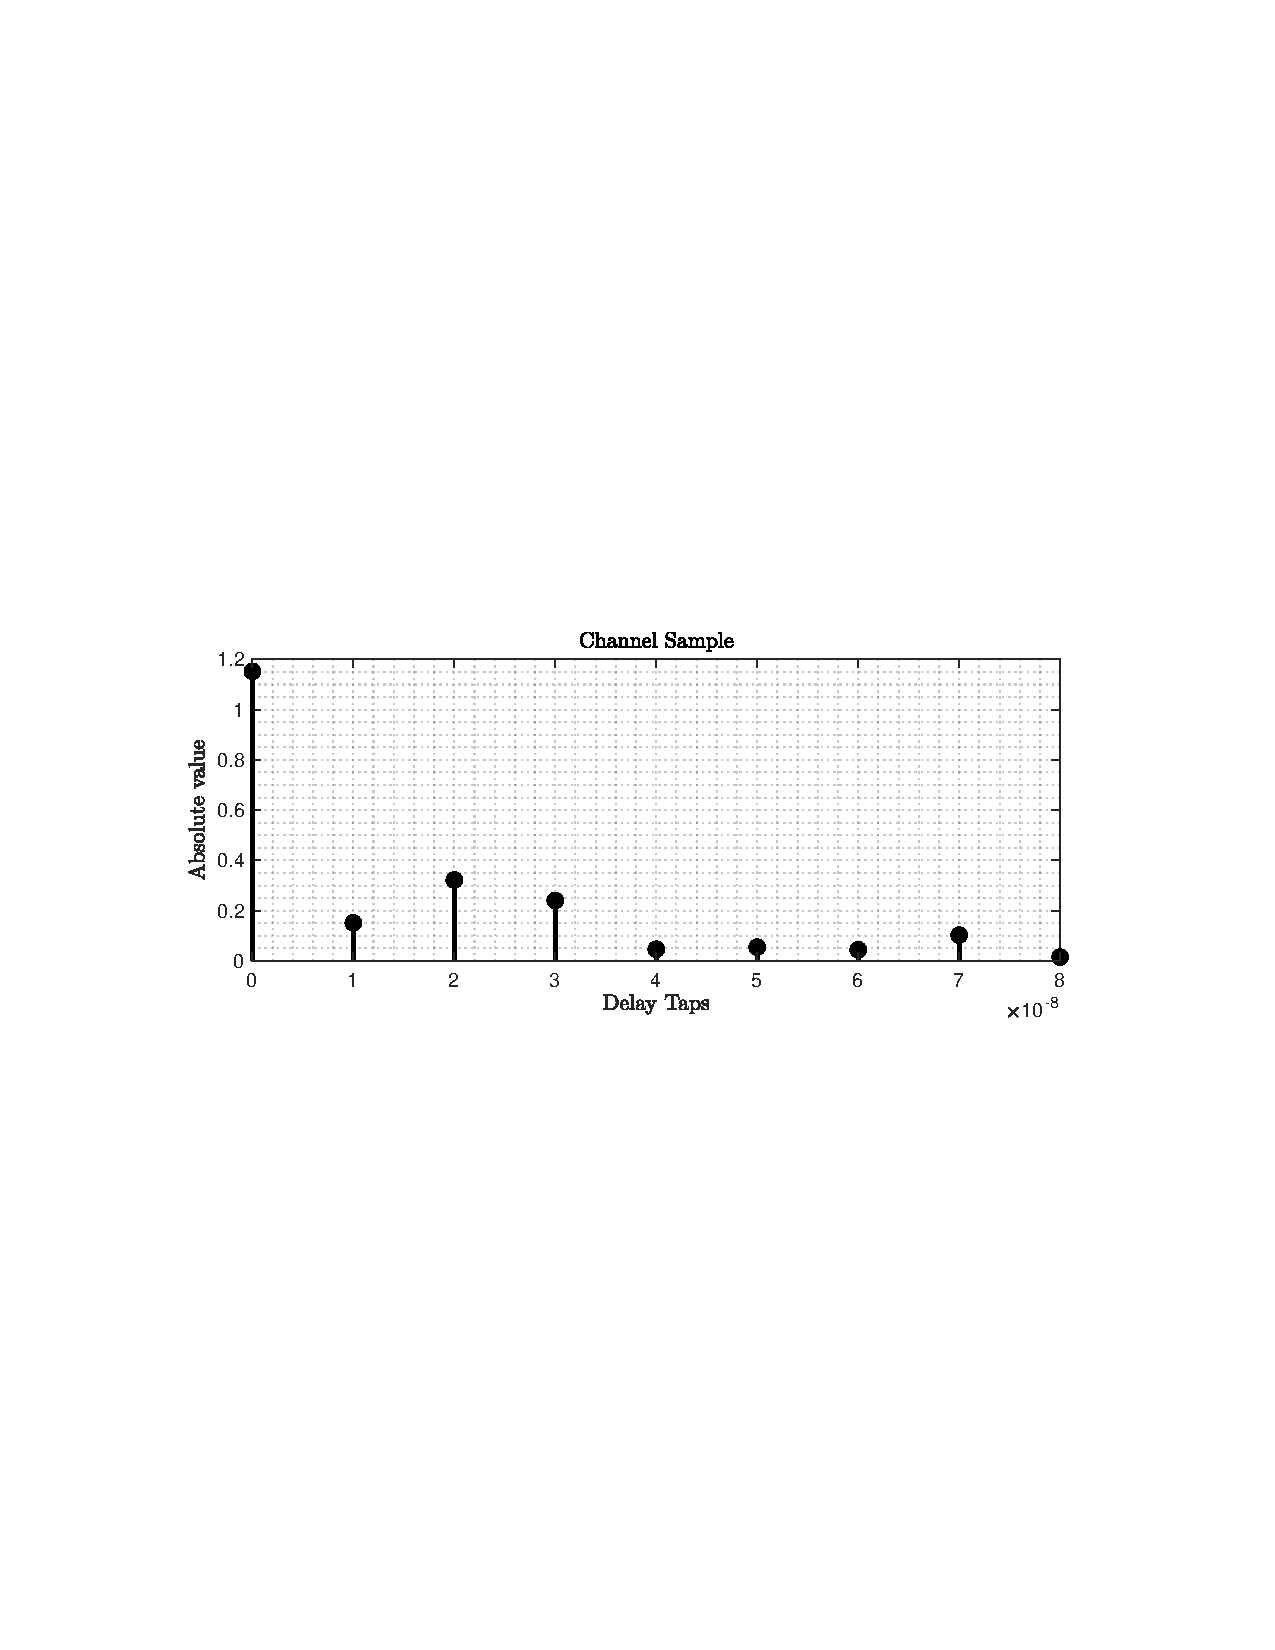
\includegraphics[height = 10cm]{figures/TimeSample.pdf}
%     \caption{Data Rate of User 1 versus its Distance from AP for Single Antenna Per User}
%     \label{fig:data-rate-distance-single}
% \end{figure}

% \begin{figure}
%     \centering
%     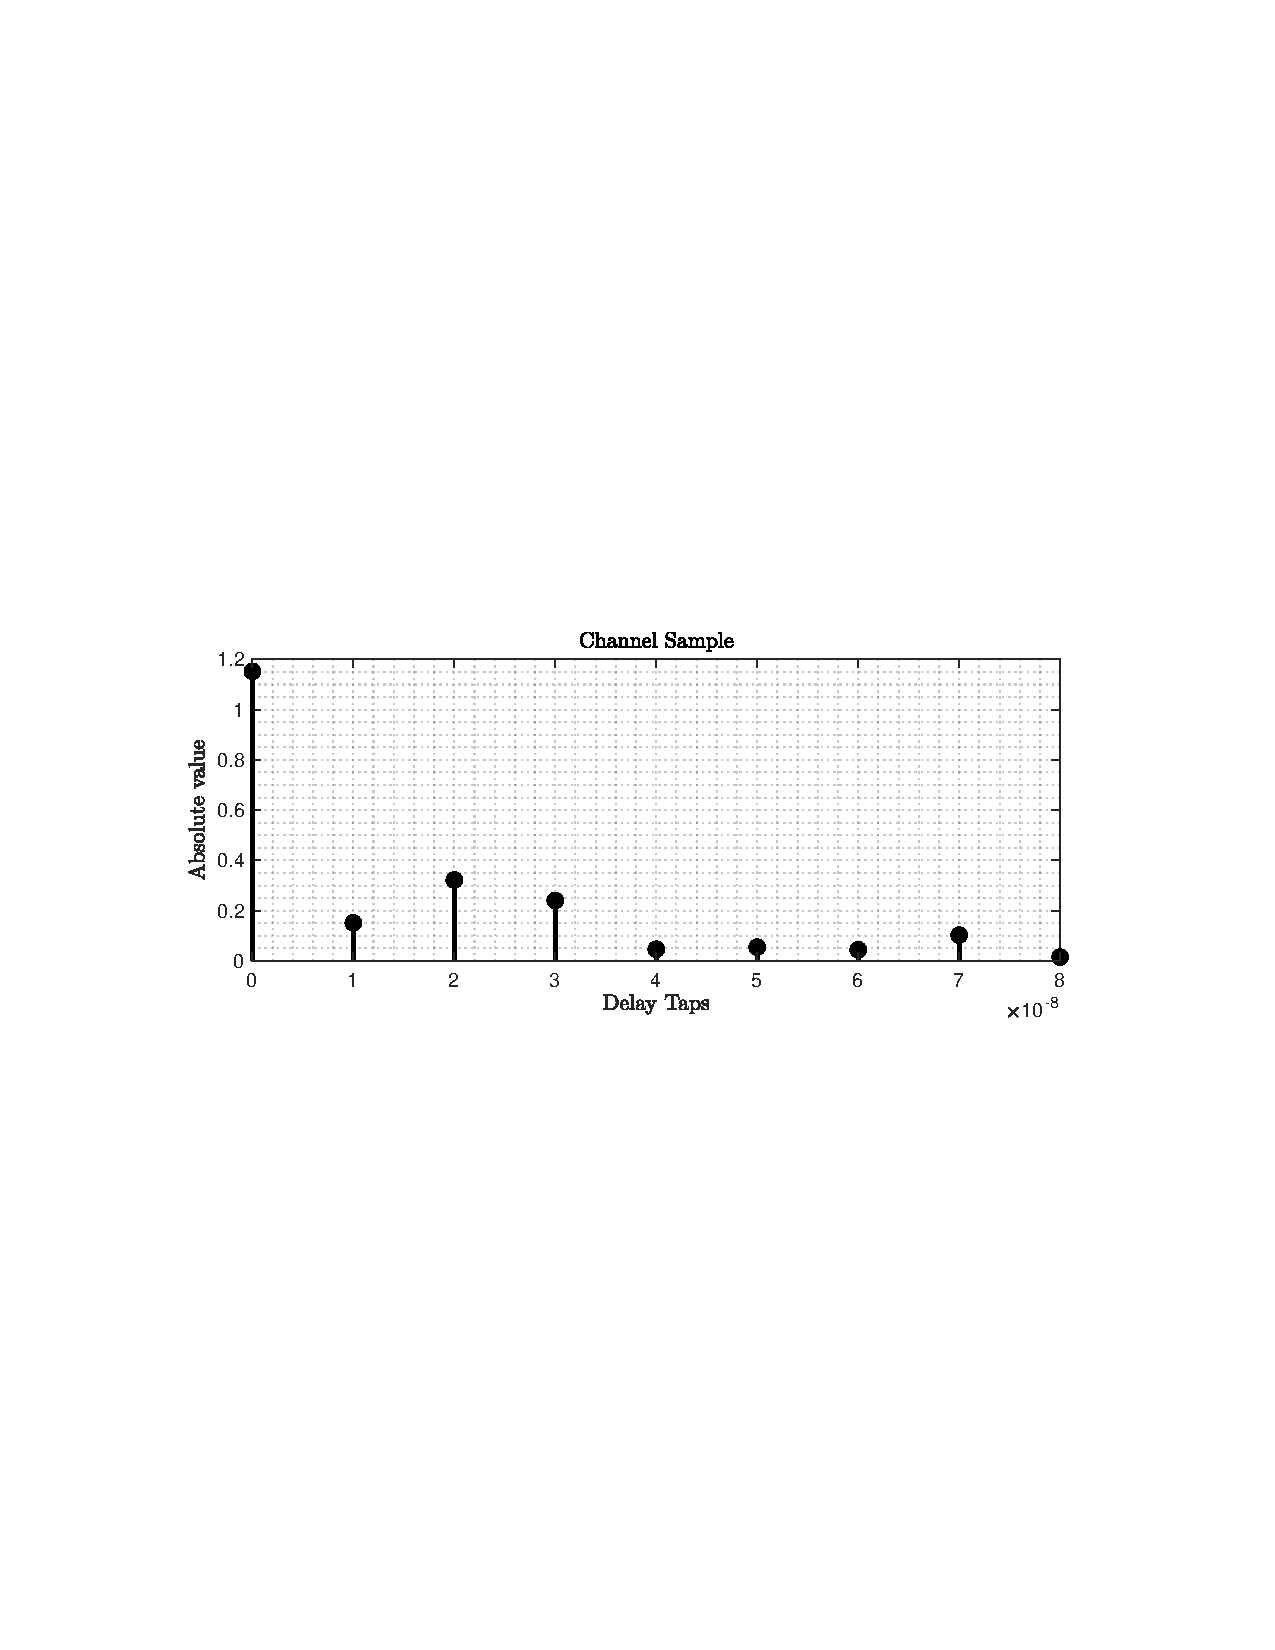
\includegraphics[height = 10cm]{figures/TimeSample.pdf}
%     \caption{Data Rate versus Number of AP antennas}
%     \label{fig:data-rate-AP-antennas-single}
% \end{figure}

% \begin{table}[t]
%     \caption{Experiment Scenarios for Multiple Antennas Per User}
%     \centering
%     \begin{tabular}{|c|c|}
%     \hline
%        & \\
%        & \\
%        & \\
%        & \\
%        &
%     \end{tabular}
%     \label{tab:scearios-multi}
% \end{table}

% \begin{figure}
%     \centering
%     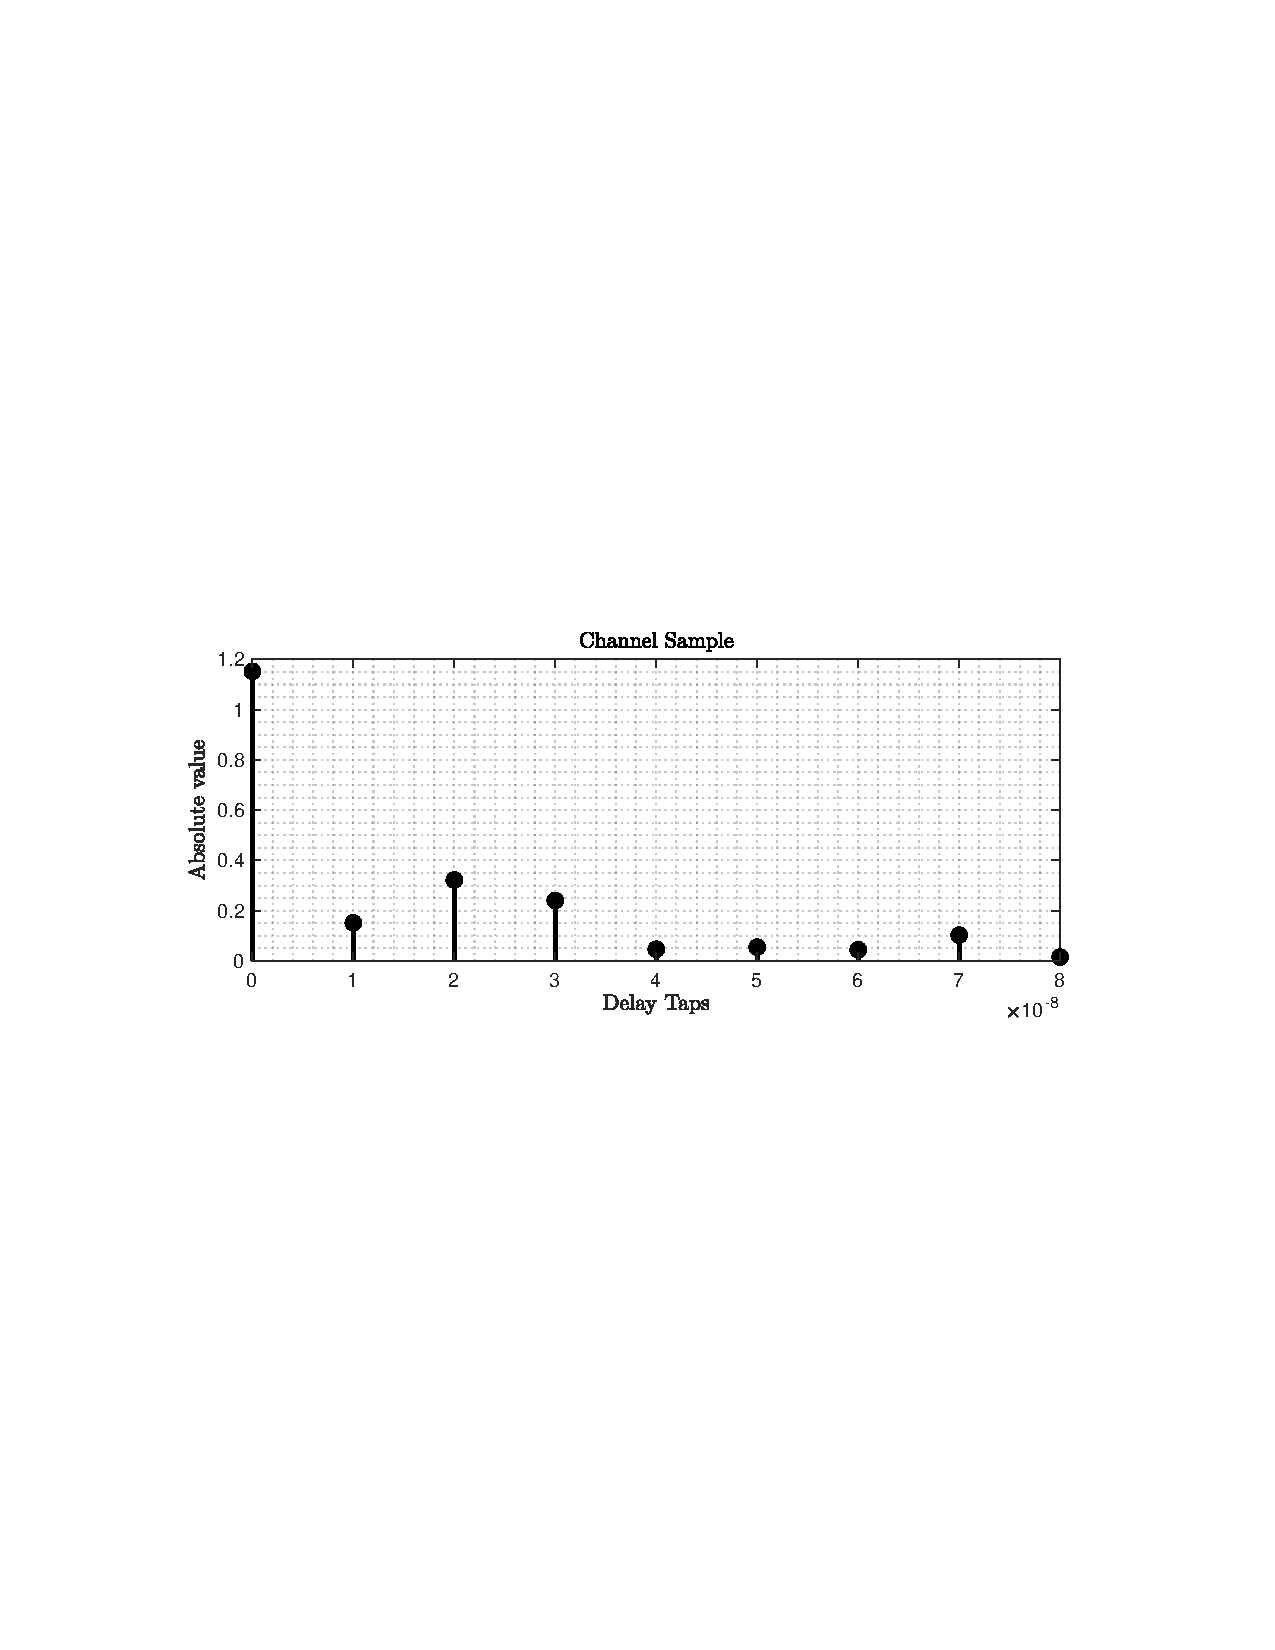
\includegraphics[height = 10cm]{figures/TimeSample.pdf}
%     \caption{Data Rate versus Number of User Antennas}
%     \label{fig:data-rate-user-antennas-multi}
% \end{figure}

% describe simulation environment: provide tables for parameters used 
In our experimental setup, we simulate a virtual reality (VR) gaming environment involving \( N \) users, each engaging in a distributed rendering task. These users, equipped with VR glasses, receive fragmented visual perspectives of a virtual room. We define \( L_{xu} \) as a 1x\( N \) array, representing the number of antennas at each user's device. Additionally, the access point (AP) is equipped with \( L_y \) antennas. The spatial positioning of users relative to the AP is modeled through a uniform random distribution, with distances ranging between \( d_{\text{min}} \) and \( d_{\text{max}} \). For the characterization of channel impulse responses between user devices and the AP, we utilize a dataset of over 10,000 channel realizations provided by Samsung. These realizations are based on WiFi 802.11ax standards \cite{802.11ax}, specifically tailored for model B (indoor residential) and model D (indoor office) scenarios. At any given moment, our experimental framework randomly selects one of these channel impulse responses for each pairing of the user device antenna and AP antenna. We multiply an additional components for path loss and shadow fading. We use the following combination of path loss and shadow fading loss:
\begin{equation}
    \begin{aligned}
        L(d) &= L_{path}(d) + L_{shadow}(d) \quad \textrm{dB}  \qquad \qquad d \leq d_{break} \\
    &= L_{path}(d_{break}) + L_{shadow}(d_{break}) + \\ & \qquad \qquad \qquad 35 \: \operatorname{log}_{10}(\frac{d}{d_{break}}) \quad \textrm{dB}  \qquad d>d_{break}
    \end{aligned}
\end{equation}
where the break-point distance is $d_{break} = 5\:m$, and 
\begin{align}
    L_{path} =  20 \: \operatorname{log}_{10}(f) + 20\: \operatorname{log}_{10}(d)  - 147.5 \textrm{dB}
\end{align}
and $L_{shadow}$ is a random log-normal variable sampled from $\frac{1}{\sqrt{2 \pi \sigma^{2}_{z}}}\exp{-(L_{shadow}(d)^{2}/(2\sigma^{2}_{z}))}$, $\sigma_{z}$ is $3 \textrm{dB}$ before breakpoint distance and $4 dB$ after the breakpoint. The channel delay taps are spaced 10 ns apart, hence the channel bandwidth is 100 MHz. In our experiments,we use the center frequency $f_{c}=5 GHz$ and vary the Fast Fourier Transform length $(fft_{length})$. Fig.~\ref{fig:channel-samples} shows an instance of the channel impulse responses used in the experiments. The parameters used for the experiments are tabulated in Table~\ref{tab:experiment-parameters}. We vary the transmit Signal-to-Noise Ratio (SNR) values and assess the resultant data rates achieved by both the baseline OFDM-based system and our proposed GDFE-based algorithm. Conversely, by setting variable minimum required data rates, we evaluate and compare the power consumption metrics for both the proposed algorithm and the baseline system. The ranges over which each of these parameters is varied are systematically tabulated for clarity and ease of reference.

% provide table and graph for results
Table \ref{tab:scearios-single} shows 2 instances of the experiment results using varying parameters. As we see from the first column, for the same data rates, the proposed algorithm consumes an order of magnitude less relative energy as compared to OFDM baselines. This shows that, even in the case where the total number of antennas at all users (2) is equal to the total number of antennas at the AP (2), harsh channel conditions and crosstalk between the subchannels lead to significant energy savings compared to OFDM, when using the proposed non-linear feedback-based algorithm. The second column stresses the channel further, i.e. forces it into a low-rank situation where the total number of antennas at the users (3) is less than the total number of antennas at the AP (2). Row lank regimes are where we see the massive benefit of using GDFE-based power allocation. This is aided by time sharing between users and thus simultaneous power allocation in the same time and frequency slot, which OFDM is incapable of. We achieve, on an average, 2 times the data rate at half the energy requirement.

Table~\ref{tab:energy-compare} demonstrates the proposed algorithm's superiority over the baseline OFDM in power efficiency across various AP antenna counts, maintaining a fixed data rate of 200 Mbps/user. The power savings become more pronounced as AP antennas decrease, attributed to the channel's lower rank in these scenarios, highlighting the algorithm's effectiveness in energy conservation under channel constrains. For the last row, where the number of antennas at AP (4) exceeds the number of user antennas (3), we see that the GDFE-based algorithm takes advantage of the crosstalk in the channel and achieves the required data rates at significantly lower energy compared to OFDM. 

Fig.~\ref{fig:data-rate-snr-single} shows the sum rate across 3 users located at equal distances of 3 m from the AP, as a function of SNR (dB). We see that the slope of increase of the data rates for the proposed algorithm is significantly higher than that for the OFDM-based current Wi-Fi algorithm. The inability of the OFDM-based system to utilize crosstalk between the channels is evident, and this crosstalk is utilized by the proposed algorithm to achieve high data rates, especially at high SNR values. There is time sharing between the three users. The first user has to suffer in data rates by treating the other two user's signals as noise, and the second user does this for the third user's signal. However, the third user gets to fully exploit all the available dimensions, which contributes to the high data rates. 

Fig.~\ref{fig:data-rate-fft-single} and Fig.~\ref{fig:data-rate-farthest-fft-single} compare the spectral efficiencies of a proposed algorithm against current Wi-Fi OFDM in equidistant users (3m, 3m, 3m) and non-equidistant users (3m, 5m, 8m) scenarios. As per Fig.~\ref{fig:data-rate-fft-single}, the proposed algorithm achieves 15 bits/s/Hz sum rates (500 Mbps/user) with FFT lengths ≥1024, outperforming OFDM's 11 bits/s/Hz. In Fig.~\ref{fig:data-rate-farthest-fft-single}, i.e., in non-equidistant setups, it ensures even the farthest user achieves equal data rates despite higher path losses, leveraging GDFE-based noise cancellation and time-sharing. The OFDM algorithm, which uses the water-filling algorithm for power allocation, fails to achieve this and hence the farthest user has the worst data rates of 2.3 bits/s/Hz at saturation. This demonstrates the proposed solution's superiority in energy and data rate efficiency, especially in low-rank channel conditions, making it a promising alternative to current Wi-Fi standards.